% @author Arian Helberg

\chapter{Einleitung}

\gls{ac:haw}~\gls{sy:ohm}~\gls{gl:haw}(Damit das glossar keine fehler schmeißt)

Effizientes Objektdesign und -modellierung sind entscheidende Kernkompetenzen in verschiedenen Bereichen der
digitalen Welt.
Da die Erstellung geometrischer Objekte für Laien unintuitiv ist und ein großes Maß an Erfahrung und Expertise
erfordert, ist dieses stetig wachsende Feld für Neueinsteiger nur sehr schwer zu erschließen.
Die Forschung liefert hierzu einige Arbeiten zur prozeduralen Modellierung, um digitale Inhalte schneller
und automatisiert zu erstellen.
Gerade wenn es um die Darstellung natürlicher Umgebung geht, ist die Erstellung von ähnlichen Objekten, wie
zum Beispiel verschiedene Bäume derselben Gattung eines Waldes, ein schwieriges Problem.
Kleine Änderungen in prozeduralen Systemen können zu großen Veränderungen der Ergebnisse führen.
Darum beschäftigt sich die inverse prozedurale Modellierung unter anderem mit dem Inferieren von Regeln
und Mustern aus gegeben Objekten, um diese nach bestimmten Regeln zu modellieren.
Ein wichtiges Werkzeug hierbei ist die Verwendung formaler Grammatiken als fundamentale Datenstruktur
der Informatik, um Strukturen zu beschreiben.
Eine spezielle Untergruppe sind die L-Systeme, die häufig bei der Beschreibung
von Verzweigungsstrukturen und Selbstähnlichkeit zum Einsatz kommen.
\\~\\
Diese Arbeit soll sich mit der Erstellung eines prozeduralen Systems zur Synthese von Ähnlichkeitsabbildern
beschäftigen.
Hierzu soll über eine Benutzerschnittstelle eine Struktur erzeugt werden, aus der ein parametrisiertes L-Systems
inferiert werden kann, das dann zur Generierung von ähnlichen Strukturen genutzt werden kann.

\newpage

\section{Problemstellung}

Mit der Digitalisierung der Welt steigt auch der Bedarf an digitalen Inhalten.\\
(Das umfasst Gaming, Unterhaltungsindustrie, Visualisierung, Interaktive Anwendungen)\\
Um eine erhöhte Quantität dieser Inhalte liefern zu können, werden Methodiken und Algorithmen gesucht, die die Erstellung
vereinfachen.
Während Methodiken zur Kodifizierung bestimmter Strukturen diese für die prozedurale Modellierung nutzbar machen,
findet das Ableiten von Regeln Anwendung in der inversen prozeduralen Modellierung.\\
Weiter steigt mit dem digitalen und naturwissenschaftlichen Fortschritt die Anwendung immer komplexerer (organisiert)
Strukturen aus der Natur (Bsp).\\
(Im Gaming-Bereich zB. gab es bisher unorganisierte Modelle aus Dreiecken. Mit besserer Graphik ist die Organisierung der
Modelle immer wichtigen, um diese effizient und automatisiert modellieren zu können; Wichtig ist auch die Wiederverwendbarkeit
der Modelle)\\
Deshalb werden allgemeingültige, vielseitig anwendbare Algorithmen gesucht, die bestimmte natürliche Eigenschaften
herausarbeiten, um diese für die (inverse) prozedurale Modellierung zur Verfügung zu stellen.
\\~\\

\\~\\
Diese Arbeit soll zeigen, wie sich durch die Erstellen eines Systems zur Generierung von ähnlichen Strukture aus einer
Basistruktur aktuelle Ansätze aus der Forschung in einem Programm umsetzen lassen.





Beschreibung eines Forschungsproblems, das ich mit der Bachelorarbeit lösen möchte.

\begin{itemize}
    \item Das Problem ist die Erstellung eines Systems zur Erzeugung von ähnlichen Strukturen aus einer Basisstruktur
    \item Der Sprung der prozeduralen Modellierung zur inversen prozeduralen Modellierung, also die Vereinfachung von schwierigen,
    schwer zu kontrollierenden prozeduralen Regeln zu einem "`Reverse Engineering"'-Ansatz (Automatisierung)
\end{itemize}

Wo besteht das Problem?

\begin{itemize}
    \item (Inverse) prozeduralle Modellierung ist ein schwieriges Problem der Informatik $\rightarrow$ Quellen sichen und
    begründen warum das so schwierig ist (\cite{aliaga_2016})
    \item Prozedurale Regeln sind schwer zu verstehen und kontrollieren $\rightarrow$ Zugang, Klarheit schaffen, wie man an
    solche Fragestellungen herangeht
    \item Schwierigkeit den Expansionsprozess zielgerichtet zu kontrollieren~\cite{prusinkiewicz_1990}
\end{itemize}

Wie wichtig ist es, dass ich meine Forschung durchführe?

\begin{itemize}
    \item Kodifizierbar machen von Strukturen der realen Welt $\rightarrow$ Künstliche Intelligenz,  Wiederverwendbarkeit,
    Umsetzten gewisser Erwartungen eines Users an eine digitale Struktur
    \item Kompression von Strukturen $\rightarrow$ Speicherkomplexität in Laufzeitkomplexität umwandeln.
    Effiziente Balance schaffen
    \item Da prozedurale Modellierung eines der mächtigsten Mittel ist, um automatisch digitale Inhalte zu Erstellen und die
    digitale Welt immer wichtiger wird, ist die Forschung in diesem Bereich sehr wichtig
    \item
\end{itemize}

Wie gut lassen sich Ansätze aus der aktuellen Forschung in einem Programm umsetzen?
\begin{itemize}
    \item Man braucht verschiedenen Algorithmen mit verschiedenen Metriken, um eine Struktur "`auslesen"' zu können, besser sind
    neuronale Netze $\rightarrow$ Quellen
\end{itemize}

Gibt es allgemeingültige Algotihmen?

\begin{itemize}
    \item Eigene Algorithmen checken, Alternativen nachschauen, sind die verwendeten Algorithmen zu sehr auf mein Problem
    zugeschnitten?
\end{itemize}

Gibt es Widersprüche in aktueller Forschung?

\begin{itemize}
    \item Nochmal einige Quellen lesen. Ich denke, es gibt keine direkten Widersprüche, aber viele verschiedene Ansätze
    $\rightarrow$ Quellen
\end{itemize}

Verbindung zum Titel der Bachelorarbeit schaffen.

\begin{itemize}
    \item Zeigen, wie ich die Synthese anhand des Programms umsetzen will
\end{itemize}

\section{Ziele}
Gewichtungsparameter durchtesten, um zu schauen, wie sich das auf die Ergebnisse auswirkt.\\
Ergebnis des Systems mit validem Input mit Ergebnissen aus nicht validem Input vergleichen, um zu schauen, wie wichtig
die Validiität des Inputs ist.\\

\section{Methodik}

\textit{Abbildung 1 zeigt, wie das o.g. System aufgebaut ist}:
\begin{itemize}
    \item[I.] \underline{Strukturieren}: Der Benutzer nutzt die grafische Benutzerschnittstelle, um aus
    einzelnen, atomaren Strukturen (\textbf{Templates}) eine zusammenhängende Struktur zu erstellen.
    Neben der Position der Templates können auch Parameter wie Rotation angepasst
    werden.
    \item[II.] \underline{Visualisieren}: Das Ergebnis der Strukturierung ist jederzeit sichtbar.
    Einfache Liniensegmente können mit einem \textbf{Turtle-Algorithmus} gezeichnet werden.
    \item[III.] \underline{Datengenerierung}: Das Ergebnis der Strukturierung wird in einer Baumstruktur
    organisiert, in der jeder Knoten einem bestimmten Template entspricht und die zugehörigen Kanten die
    geometrischen Transformationen relativ zum Elternknoten beschreibt.
    \item[IV.] \underline{Inferieren}: Aus der Baumstruktur kann eine formale Grammatik in Form eines kleinen
    L-Systems abgeleitet werden, indem identische topologische Strukturen (Unterbäume) gefunden werden können.
    \item[V.] \underline{Optimieren}: Hier werden ähnliche Produktionsregeln des L-Systems mithilfe einer
    \textbf{Kostenfunktion}\footnote[1]{Die Kostenfunktion setzt sich sowohl aus der Länge der Grammatik, als
    auch der Distanz von der alten zur neuen, generalisierten Grammatik nach dem Merge zusammen} zusammengefasst
    (\textit{engl. Merge}), um diese mit nicht-deterministischen Regeln und Rekursion zu generalisieren.
    \item[VI.] \underline{Randomisieren}: Jedes Symbol der Grammatik nimmt eine Liste an Parametern entgegen, die
    in diesem Schritt nach bestimmten Kriterien pseudo-randomisiert werden, um Variationen zu erstellen und
    anschließend zu visualisieren.
\end{itemize}

\section{Aufbau}

Im Folgenden wird auf die Methodik zum Ableiten eines L-Systems eingegangen und Konzepte und eigene Lösungsansätze
präsentiert.

\begin{figure}[H]
    \centering
    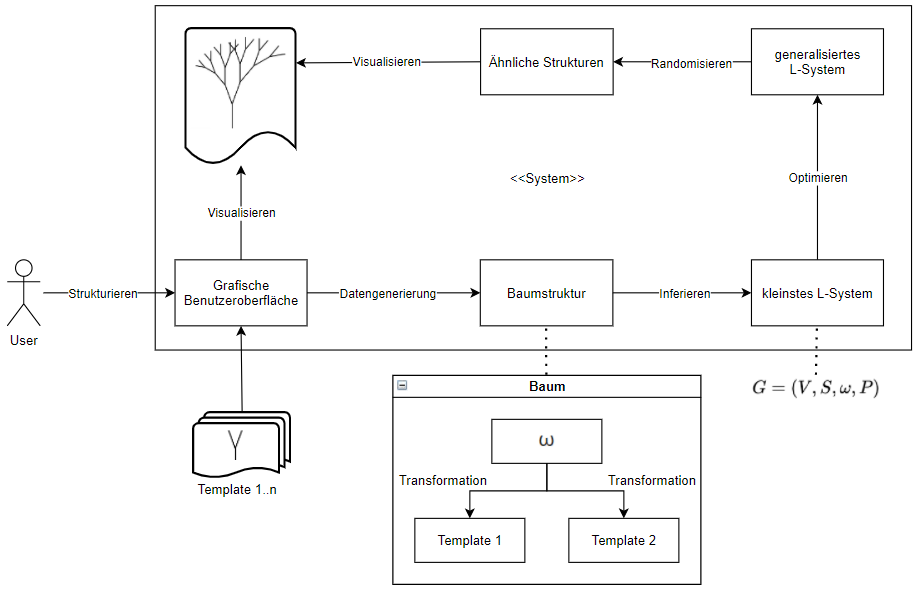
\includegraphics[width=14cm]{../images/System.PNG}
    \caption[Systemarchitektur]{Architektur des Systems mit einigen Datenstrukturen}
\end{figure}

\subsubsection{System}
Ziel des Systems ist die Erstellung von Ähnlichkeitsabbildern einer Struktur, die über eine grafische
Benutzeroberfläche erstellt wird.